\noindent

\includegraphics[height=1.25cm]{images/pictograms/benchmark}

\includegraphics[height=1.25cm]{images/pictograms/tools}

\includegraphics[height=1.25cm]{images/pictograms/FEM}

\includegraphics[height=1.25cm]{images/pictograms/paraview}


%%%%%%%%%%%%%%%%%%%%%%%%%%%%%%%%%%%%%%%%%%%%%%%%%%%%%%%%%%%%%%%%%%%%%%%%%%%%%%%%%%%%%%%%%%%%%%%%%%%

\begin{flushright} {\tiny {\color{gray} python\_codes/fieldstone\_250/text.tex}} \end{flushright}

\lstinputlisting[language=bash,basicstyle=\small]{python_codes/fieldstone_150/keywords.key}

\par\noindent\rule{\textwidth}{0.4pt}

\begin{center}
\inpython
{\small Code: \url{https://github.com/cedrict/fieldstone/tree/master/python_codes/fieldstone_150}}
\end{center}

\par\noindent\rule{\textwidth}{0.4pt}

%%%%%%%%%%%%%%%%%%%%%%%%%%%%%%%%%%%%%%%%%%%%%%%%%%%%%%%%%%%%%%%%%%%%%%%%%%%%%%%%%%%%%%%%%%%%%%%%%%%

This \stone is an attempt at looking into the optimisation of how (FE) stones have been coded 
up until now. In particular I want to try to build the (Stokes) FE matrix much faster.
If successful, this would enable either higher resolution runs, or longer time series, 
or a quicker way to steady state, etc ...

We then start from the {\pythonfile stone\_V0.py} script which solves the 
Donea \& Huerta benchmark (see \ref{mmm:mms1}) in a unit square by means of \QtwoQone elements.
It is very similar to \stone~\ref{f48} for example.

%%%%%%%%%%%%%%%%%%%%%%%%%%%%%%%%%%%%%%%%%%%%%%%%%
\section*{Standard approach}

Running the model at resolution $128 \times 128$ elements, we find that building 
the matrix takes approximately 11.7s and solving the system approximatively 1.4s.  
Although the solve time grows like $nel^{1.66}$, even running a $256\times 256$ elements model 
would still yields a build time that is substantially larger than the solve time.
Also, the part of the code which computes the $L_2$ errors can take up to a 
few seconds (in general 10x less time than building the matrix).
This is reason enough to try to make building the matrix {\it much} faster.
Although there is no hard rule, it is commonly accepted that the solve is the 
most expensive part of a Stokes FE code.

\begin{center}
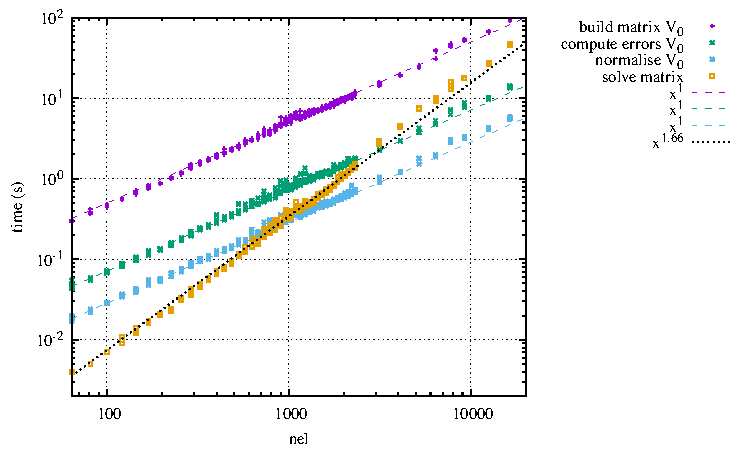
\includegraphics[width=8.5cm]{python_codes/fieldstone_150/results/times_V0}
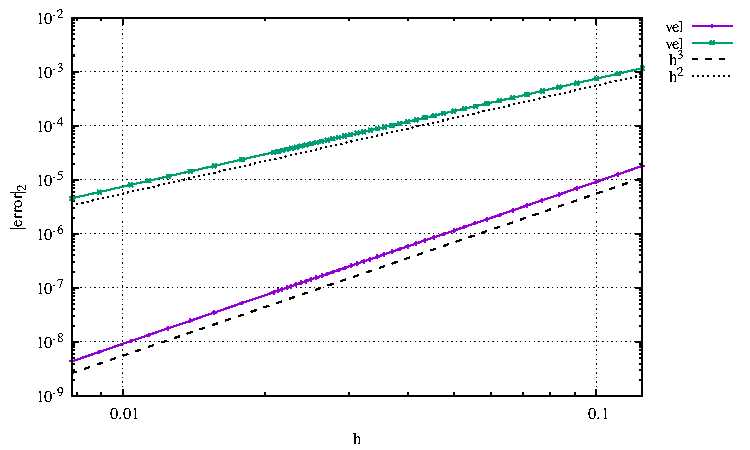
\includegraphics[width=8.5cm]{python_codes/fieldstone_150/results/errors_V0}\\
{\captionfont 
Left: Timings of 4 parts of the code as a function of the number of elements.
Right: $L_2$-error convergence plot as a function of the element size $h$.
}
\end{center}



%%%%%%%%%%%%%%%%%%%%%%%%%%%%%%%%%%%%%%%%%%%%%%%%%
\section*{Dealing with the Jacobian matrix code bits}

To start with I here assume that we are dealing with rectangular elements, 
all of the same size $(h_x,h_y)$. This allows to replace this typical piece of code 
\begin{lstlisting}
for iel in range(0,nel):
    for iq in range(0,nqperdim):
        for jq in range(0,nqperdim):
            ...
            jcb=np.zeros((ndim,ndim),dtype=np.float64)
            for k in range(0,mV):
                jcb[0,0] += dNNNVdr[k]*xV[iconV[k,iel]]
                jcb[0,1] += dNNNVdr[k]*yV[iconV[k,iel]]
                jcb[1,0] += dNNNVds[k]*xV[iconV[k,iel]]
                jcb[1,1] += dNNNVds[k]*yV[iconV[k,iel]]
            jcob = np.linalg.det(jcb)
            jcbi = np.linalg.inv(jcb)
\end{lstlisting}
by something much simpler. Indeed, in this case the Jacobian matrix is 
\[
{\bm J}=\left(
\begin{array}{cc}
h_x/2 & 0 \\ 0 & h_y/2
\end{array}
\right)
\]
so that the determinant is $|{\bm J}|=h_xh_y/4$ and its inverse:
\[
{\bm J}^{-1}
=\left(
\begin{array}{cc}
2/h_x & 0 \\ 0 & 2/h_y
\end{array}
\right)
\]
We can then replace the code excerpt above (which is usually called at every quadrature 
of every element) by:
\begin{lstlisting}
jcbi=np.zeros((ndim,ndim),dtype=np.float64)
jcbi[0,0]=2/hx
jcbi[1,1]=2/hy
jcob=hx*hy/4

for iel in range(0,nel):
    for iq in range(0,nqperdim):
        for jq in range(0,nqperdim):
            ...

\end{lstlisting}
Note that the explicit calculation of the Jacobian determinant and inverse
is also present in the pressure normalisation and error calculations.

This is very simple and 
is carried out in {\pythonfile stone\_V1.py}.

\begin{center}
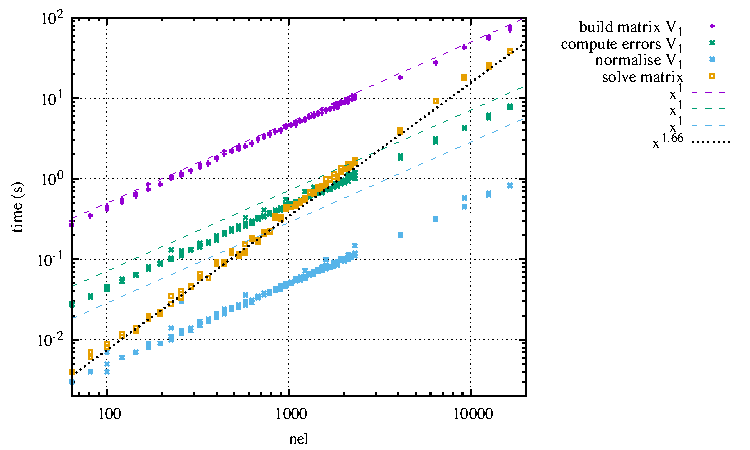
\includegraphics[width=8.5cm]{python_codes/fieldstone_150/results/times_V1}\\
{\captionfont Timings of 4 parts of the code as a function of the number of elements.
The dotted lines correspond to the timings of version V0.}
\end{center}

\begin{center}
\begin{tabular}{lcc}
\hline
& V0 & V1 \\
\hline
\hline
build matrix      ($128\times 128$)& 77.3-82.4 s&  69.7-78 s \\
normalise pressure($128\times 128$)&           s&  0.81-0.84 s\\
compute errors    ($128\times 128$)& 12.2-12.9 s& 7.6-8 s    \\
\hline
\end{tabular}
\end{center}

We see that this change has not really lead to a substantial improvement in 
computational time, especially for the build time (only 10\% improvement)... 



%%%%%%%%%%%%%%%%%%%%%%%%%%%%%%%%%%%%%%%%%%%%%%%%%
\section*{Dealing with the basis functions}

In about every FE code so far, we encounter this bit:

\begin{lstlisting}
NNNV    = np.zeros(mV,dtype=np.float64) 
NNNP    = np.zeros(mP,dtype=np.float64) 
dNNNVdr = np.zeros(mV,dtype=np.float64) 
dNNNVds = np.zeros(mV,dtype=np.float64) 

for iel in range(0,nel):
    for iq in range(0,nqperdim):
        for jq in range(0,nqperdim):
            rq=qcoords[iq]
            sq=qcoords[jq]
            weightq=qweights[iq]*qweights[jq]

            NNNV[0:mV]=NNV(rq,sq)
            dNNNVdr[0:mV]=dNNVdr(rq,sq)
            dNNNVds[0:mV]=dNNVds(rq,sq)
            NNNP[0:mP]=NNP(rq,sq)
\end{lstlisting}
If we look at it more closely, we see that the basis functions are evaluated for every 
element at the (here) 9 reduced coordinates of the quadrature points. 
We should then instead precompute the values of the basis functions at the 
reduced coordinates of the {\tt nqel}={\tt nqperdim**ndim} quadrature points as follows:

\begin{lstlisting}
NNNV    = np.zeros((nqel,mV),dtype=np.float64) 
NNNP    = np.zeros((nqel,mP),dtype=np.float64) 
dNNNVdr = np.zeros((nqel,mV),dtype=np.float64) 
dNNNVds = np.zeros((nqel,mV),dtype=np.float64) 
rq = np.zeros(nqel,dtype=np.float64) 
sq = np.zeros(nqel,dtype=np.float64) 
weightq = np.zeros(nqel,dtype=np.float64) 
   
counterq=0 
for iq in range(0,nqperdim):
    for jq in range(0,nqperdim):
        rq[counterq]=qcoords[iq]
        sq[counterq]=qcoords[jq]
        weightq[counterq]=qweights[iq]*qweights[jq]
        NNNV[counterq,0:mV]=NNV(rq,sq)
        dNNNVdr[counterq,0:mV]=dNNVdr(rq,sq)
        dNNNVds[counterq,0:mV]=dNNVds(rq,sq)
        NNNP[counterq,0:mP]=NNP(rq,sq)
        counterq+=1
\end{lstlisting}
so that we can later reuse these where needed (note that we have transformed the 
double for loop on quadrature points into a single one):
\begin{lstlisting}
for iel in range(0,nel):
    for iq in range(0,nqel):
        ...
        rq[iq],sq[iq],weightq[iq]
        NNNV[iq,0:mV]
        dNNNVdr[iq,0:mV]
        dNNNVds[iq,0:mV]
        NNNP[iq,0:mP]
\end{lstlisting}

Looking further down we then see that the inverse of the Jacobian matrix 
is used to compute the derivatives of the basis functions in the real 
coordinate space $(x,y)$:
\begin{lstlisting}
for k in range(0,mV):
    dNNNVdx[k]=jcbi[0,0]*dNNNVdr[k]+jcbi[0,1]*dNNNVds[k]
    dNNNVdy[k]=jcbi[1,0]*dNNNVdr[k]+jcbi[1,1]*dNNNVds[k]
\end{lstlisting}
From what follows above we know that {\tt jcbi[0,1]} and {\tt jcbi[1,0]} are 
both zero, so that in fact we have 
\begin{lstlisting}
for k in range(0,mV):
    dNNNVdx[k]=jcbi[0,0]*dNNNVdr[k]
    dNNNVdy[k]=jcbi[1,1]*dNNNVds[k]
\end{lstlisting}
which means that these too can be precomputed at the quadrature points before entering 
the loop over elements:
\begin{lstlisting}
NNNV    = np.zeros((nqel,mV),dtype=np.float64) 
NNNP    = np.zeros((nqel,mP),dtype=np.float64) 
dNNNVdr = np.zeros((nqel,mV),dtype=np.float64) 
dNNNVds = np.zeros((nqel,mV),dtype=np.float64) 
dNNNVdx = np.zeros((nqel,mV),dtype=np.float64) 
dNNNVdy = np.zeros((nqel,mV),dtype=np.float64) 
rq = np.zeros(nqel,dtype=np.float64) 
sq = np.zeros(nqel,dtype=np.float64) 
weightq = np.zeros(nqel,dtype=np.float64) 
 
counterq=0 
for iq in range(0,nqperdim):
    for jq in range(0,nqperdim):
        rq[counterq]=qcoords[iq]
        sq[counterq]=qcoords[jq]
        weightq[counterq]=qweights[iq]*qweights[jq]
        NNNV[counterq,0:mV]=NNV(rq,sq)
        dNNNVdr[counterq,0:mV]=dNNVdr(rq,sq)
        dNNNVds[counterq,0:mV]=dNNVds(rq,sq)
        NNNP[counterq,0:mP]=NNP(rq,sq)
        dNNNVdx[counterq,0:mV]=jcbi[0,0]*dNNNVdr[counterq,0:mV]
        dNNNVdy[counterq,0:mV]=jcbi[1,1]*dNNNVds[counterq,0:mV]
        counterq+=1

for iel in range(0,nel):
    for iq in range(0,nqel):
        ...
\end{lstlisting}
All of this now happens only once, before entering the element loop!
This means that inside the element loop and the quadrature point loop, 
only the calculation of $\K_e$, the boundary conditions and the assembly 
must take place.
In the very specific case that the viscosity is constant (at least within each element)
one could also precompute $\K_e/\eta_e$ beforehand for example. 
Another interesting option would be to compute $\K_e$ for a linear viscosity in the
element given by $\eta_e(x,y)=a+bx+cy$ (think symbolic calculation ?).

This is carried out in {\pythonfile stone\_V2.py}.








%%%%%%%%%%%%%%%%%%%%%%%%%%%%%%%%%%%%%%%%%%%%%%%%%%%%%%%%%%%%%%%%%%%%%%%%%%%%%%%%%%%%%%%%%%%%%%%%%%%
\par\noindent\rule{\textwidth}{0.4pt}

\vspace{.5cm}

\begin{center}
\fbox{\begin{minipage}{0.9\textwidth}
{\color{teal}To Do, open questions, future work?}
\begin{itemize}
\item do smthg
\end{itemize}
\end{minipage}}
\end{center}

%%%%%%%%%%%%%%%%%%%%%%%%%%%%%%%%%%%%%%%%%%%%%%%%%%%%%%%%%%%%%%%%%%%%%%%%%%%%%%%%%%%%%%%%%%%%%%%%%%%
\vspace{.5cm}

\Literature:\\
\fullcite{xxxxYY}


